\maketitle

\cleardoublepage
\phantomsection
\addcontentsline{toc}{chapter}{Indice}
\tableofcontents

\listoffigures

\chapter{Il Programma}
\section{Introduzione}
\textsl{\textbf{Climate Monitoring}} \`e un'applicazione finalizzata alla rilevazione e all'analisi di parametri climatici forniti da centri di monitoraggio sul territorio italiano, in grado di rendere disponibili, a operatori ambientali e comuni cittadini, i dati relativi alla propria zona di interesse.
\subsection{Funzionamento generale dell'applicazione}
L'applicazione offre diverse funzionalit\`a tra cui:
\begin{itemize}
	\item la creazione di nuovi centri di monitoraggio climatico;
	\item l'inserimento di nuove misurazioni con i relativi parametri climatici;
	\item la visualizzazione delle aree geografiche presenti nel database;
	\item la visualizzazione di centri di monitoraggio presenti nel database;
	\item la visualizzazione delle misurazioni presenti nel database;
	\item la visualizzazione degli operatori registrati nel database.
\end{itemize}
\pagebreak
I parametri climatici che possono essere rilevati e inseriti sono:
\begin{itemize}
	\item \textsl{Vento}, la cui velocit\`a \`e espressa in km/h;
	\item \textsl{Umidit\`a}, misurata in percentuale (\%);
	\item \textsl{Pressione}, misurata in hPa;
	\item \textsl{Temperatura}, misurata in C°;
	\item \textsl{Precipitazione}, misurata in mm di pioggia;
	\item \textsl{Altitudine dei ghiacciai}, misurata in m;
	\item \textsl{Massa dei ghiacciai}, misurata in kg.
\end{itemize}
L'intensit\`a di ogni fenomeno climatico viene misurata su una scala che va da \textbf{1} (\textsl{critico}) a \textbf{5} (\textsl{ottimale}).
Il valore \textbf{0} (\textsl{default}) è riservato a parametri non inseriti o non rilevanti per una determinata area (e.g. massa dei ghiacciai in un'area desertica).

Possono inoltre essere presenti delle note testuali (di massimo 256 caratteri) per descrivere con più precisione i dati geografici.

L'applicazione permette:
\begin{itemize}
	\item ai \textbf{\textsl{comuni cittadini}}, di visualizzare i parametri climatici di proprio interesse relativi a ciascuna area geografica;
	\item a \textbf{\textsl{operatori autorizzati}}, di gestire le aree di interesse inserendo i vari parametri climatici.
\end{itemize}
Inoltre questi ultimi hanno la possibilit\`a di registrarsi, creare nuovi centri di monitoraggio e aggiungervi aree di interesse.

\pagebreak

\chapter{Installazione}
\section{Requisiti di sistema}
Per eseguire l’applicazione \`e necessario avere a disposizione:
\begin{itemize}
	\item Java JDK 17 o superiore;
	\item un sistema operativo a 64 bit;
	\item un terminale.
	\item server PostgreSQL
\end{itemize}

\section{Setup Ambiente}

Il client richiede il server del progetto e un database PostgreSQL.

\subsection{Database}

Il database deve essere PostgreSQL.

Impostarlo correttamente è al di fuori dello scopo di questo manuale.

\subsection{Server}

Il server necessita di un database PostgreSQL gia avviato e funzionante.

Perché il server sappia dove trovare il database è necessario creare un file \texttt{postgres.env} a fianco dell'eseguibile.

\begin{lstlisting}[caption={Esempio \texttt{postgres.env}}]
POSTGRES_HOST=localhost
POSTGRES_DB=dbCM
POSTGRES_USER=postgres
POSTGRES_PASSWORD=example
\end{lstlisting}

\subsection{Client}

Il client necessita di un server gia avviato e funzionante.

Perché il client sappia dove trovare il server è necessario creare un file \texttt{config.env} a fianco dell'eseguibile.

\begin{lstlisting}[caption={Esempio \texttt{config.env}}]
RMI_HOST=localhost
\end{lstlisting}

\section{Installazione programma}

Per installare il programma:

\begin{enumerate}
	\item Scaricare da Github releases (\url{https://github.com/Qu4draetto-A3B/UniLab-client/releases}) il file adatto al proprio sistema operativo.
	\item Spostarlo dove si preferisce.
	\item Fare doppio click sul file.
\end{enumerate}

\chapter{Esecuzione e uso delle funzionalità}
\section{Lancio del programma}
All’avvio dell’applicazione compare la seguente schermata, dove è possibile visualizzare il menù principale del programma.
\section{Schermata Home}

\begin{figure}[h]
	\centering
	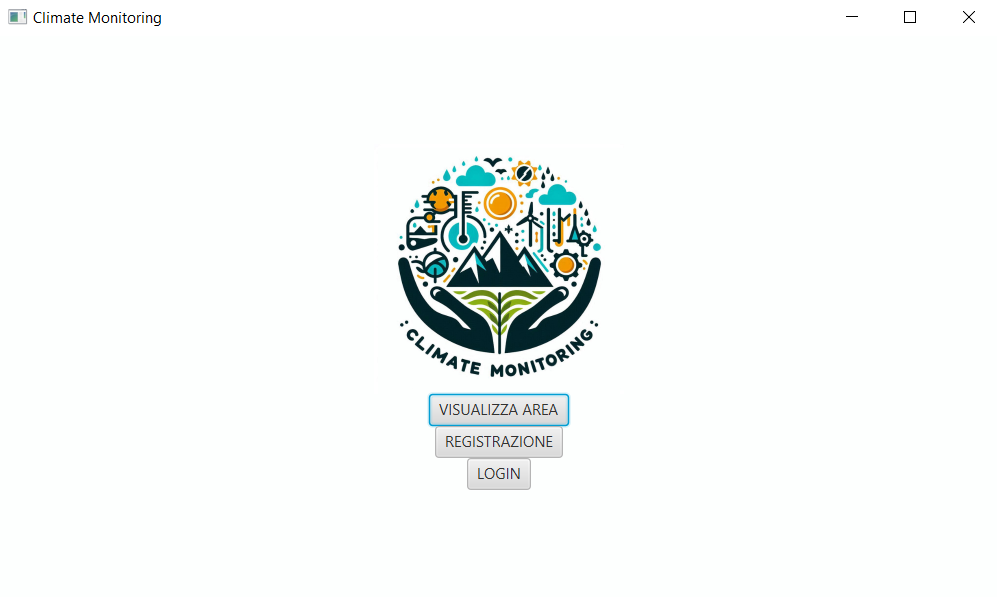
\includegraphics[height=0.3\textheight]{img/utente/home}
	\caption{Home}
	\label{fig:home}
\end{figure}

Come si può notare dall'immagine, la schermata di avvio dell'applicazione è dotata di tre pulsanti:
\begin{itemize}
	\item \textbf{\textit{Visualizza area}}, permette di visualizzare tutte le aree geografiche presenti con le relative misurazioni;
	\item \textbf{\textit{Registrazione}}, permette all'operatore di registrarsi nel sistema e accedere a una serie di funzioni a lui riservate;
	\item \textbf{\textit{Login}}: permette all'operatore già registrato di accedere al sistema. 
\end{itemize}
In tutte le schermate dell'applicazione sono presenti inoltre due pulsanti:
\begin{itemize}
	\item \textbf{freccia a sinistra}, permette di tornare alla schermata precedente;
	\item \textbf{icona della casa}, permette di tornare alla schermata Home dell'applicazione.
\end{itemize}

\subsection{Visualizza area}\label{VisualizzaArea}

\begin{figure}[h]
	\centering
	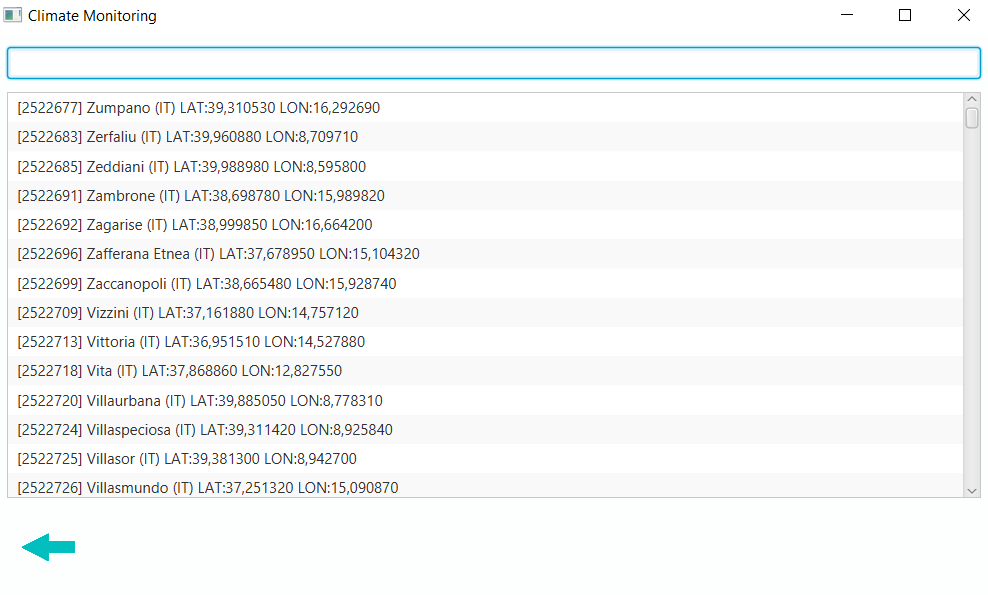
\includegraphics[height=0.3\textheight]{img/utente/SelezioneAreaGeografica}
	\caption{Visualizza area geografica}
	\label{fig:selezioneareageografica}
\end{figure}

Questa pagina presenta una barra di ricerca, dove è possibile effettuare delle ricerche sulle aree geografiche presenti nel database.

\pagebreak

Con un doppio click o selezionando l'area geografica con il mouse e premendo il tasti invio, è possibile visualizzare tutte le misurazioni relative a un'area specifica tramite un istogramma.

\begin{figure}[h]
	\centering
	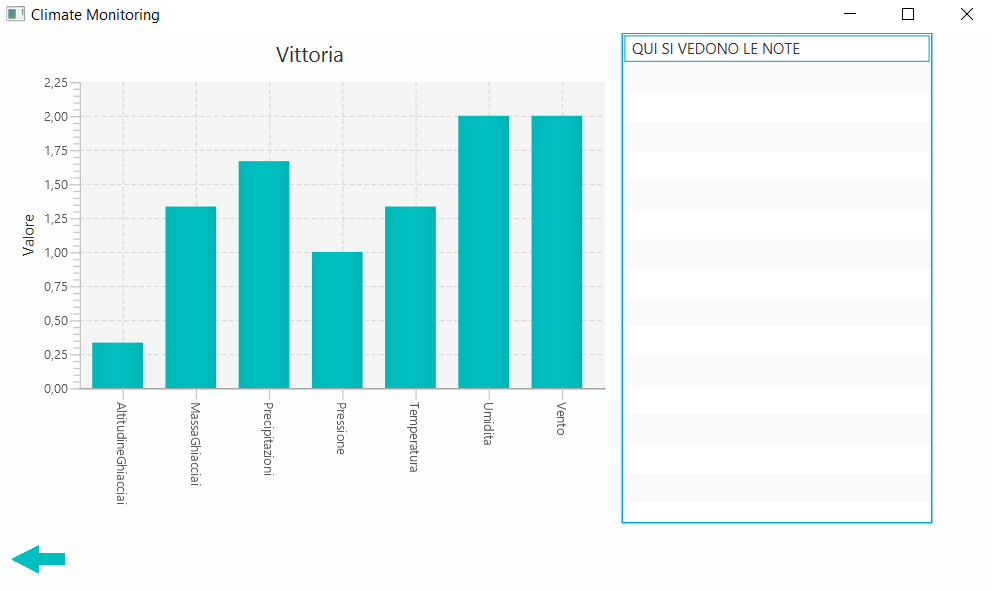
\includegraphics[height=0.3\textheight]{img/utente/VisulizzaParametro}
	\caption{}
	\label{fig:visulizzaparametro}
\end{figure}

Facendo click su una colonna dell'istogramma è possibile visualizzare le eventuali note associate.

\subsection{Registrazione}

\begin{figure}[h]
	\centering
	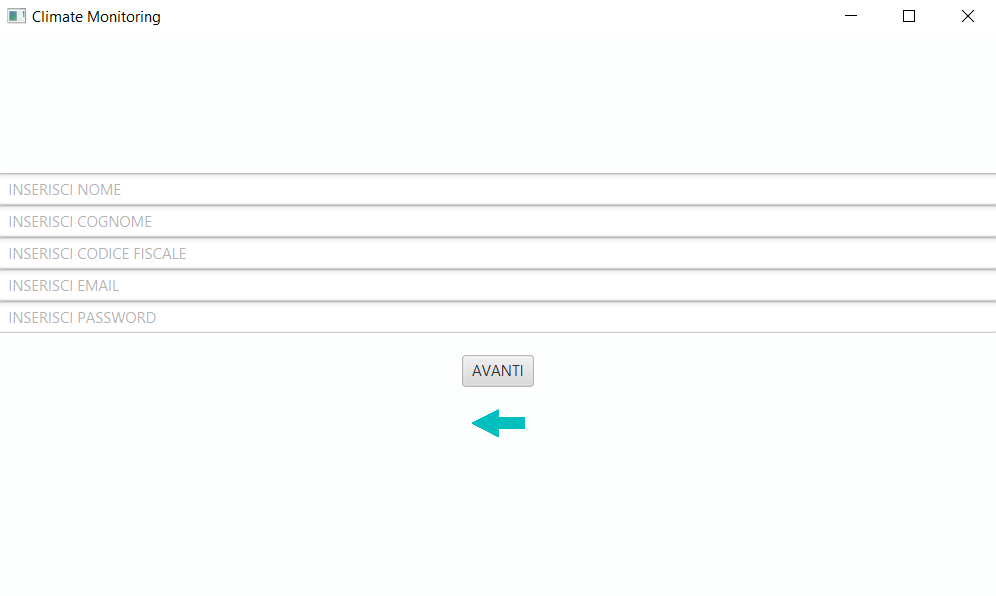
\includegraphics[height=0.3\textheight]{img/utente/Registrazione}
	\caption{Registrazione}
	\label{fig:registrazione}
\end{figure}

In questa schermata sono presenti tutti i campi che l'operatore deve compilare per la registrazione. Per la conferma è presente il pulsante \textbf{Registrazione}.

In particolare, i dati che l'operatore deve inserire sono:
\begin{itemize}
	\item  \textbf{UserID}, codice identificativo dell'utente;
	\item  \textbf{Nome};
	\item  \textbf{Cognome};
	\item  \textbf{Codice Fiscale};
	\item  \textbf{Email};
	\item  \textbf{Password}, che verrà richiesta in caso di accessi futuri.
\end{itemize}
Una volta premuto il tasto \textbf{Registrazione} viene aperta una nuova schermata, che ha lo scopo di associare un centro di monitoraggio all'operatore appena registrato.

In particolare l'operatore deve scegliere se creare un nuovo centro di monitoraggio o selezionarne uno già esistente, premendo il pulsante corrispondente.

\subsection{Operatore}
Mostra le funzioni che svolge l'operatore 
\begin{figure}[h]
	\centering
	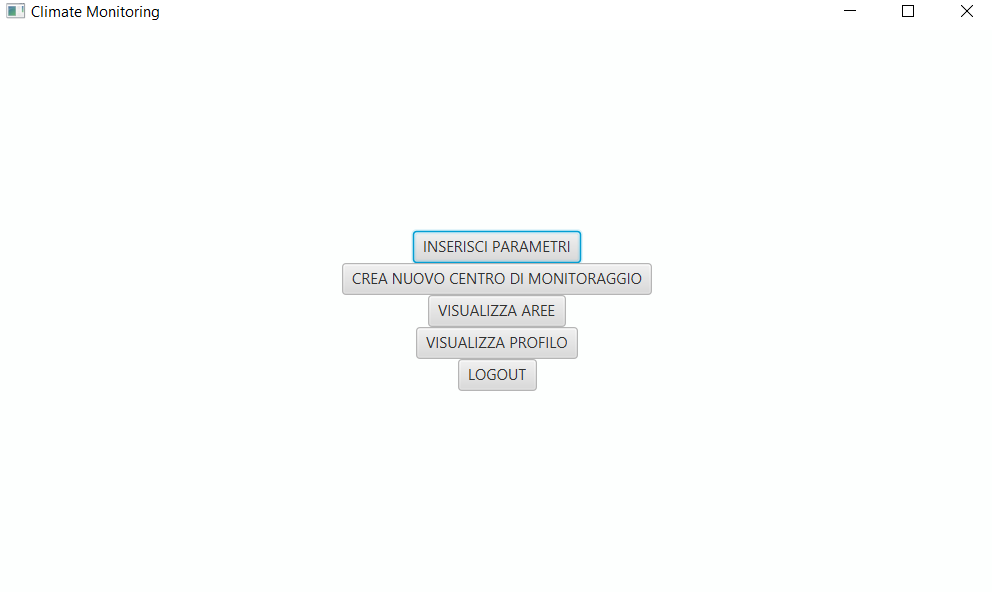
\includegraphics[height=0.3\textheight]{img/utente/SchermataOperatore}
	\caption{Operatore}
	\label{fig:schermataoperatore}
\end{figure}

\pagebreak

\subsection{Centro di monitoraggio esistente}
Questa schermata consente di far visualizzare i centri di monitoraggio esistenti.
Con un doppio-click o con un singolo click e il tasto invio seleziona il centro di monitoraggio esistente.

\begin{figure}[h]
	\centering
	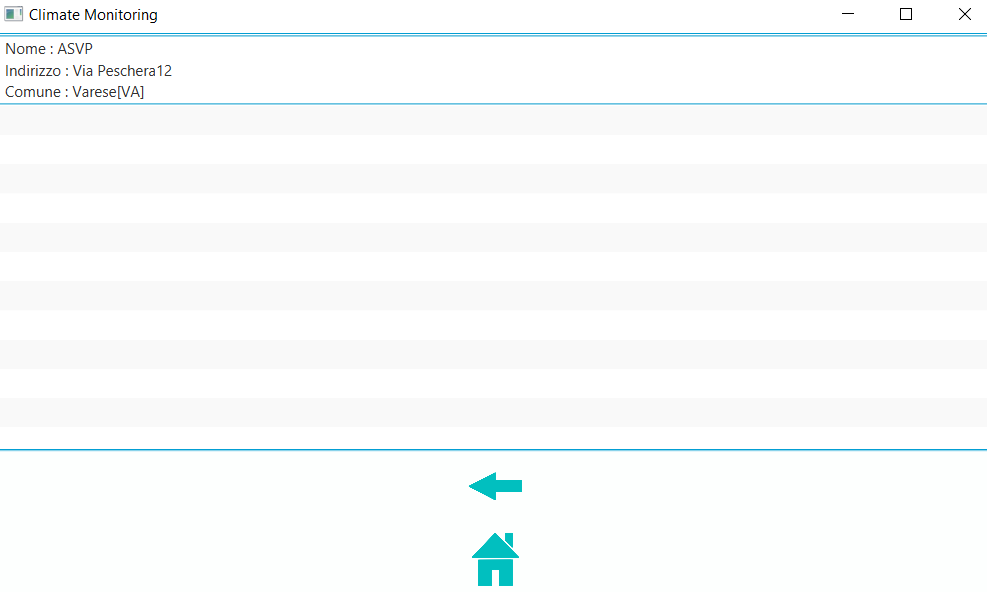
\includegraphics[height=0.3\textheight]{img/utente/CentroEsistente}
	\caption{Centro di monitoraggio esistente}
	\label{fig:centroesistente}
\end{figure}

\subsection{Nuovo centro di monitoraggio} \label{NuovoCentroDiMonitoraggio}
In caso di selezione di quest'ultimo viene aperta la seguente pagina, nella quale andranno inseriti i dati per creare un nuovo centro di monitoraggio:
\begin{itemize}
	\item \textbf{Città}
	\item \textbf{Provincia}
	\item \textbf{Via}
	\item \textbf{Numero civico}
	\item \textbf{CAP}
\end{itemize}

\pagebreak

Per la conferma è presente il relativo pulsante.
	
\begin{figure}[h]
	\centering
	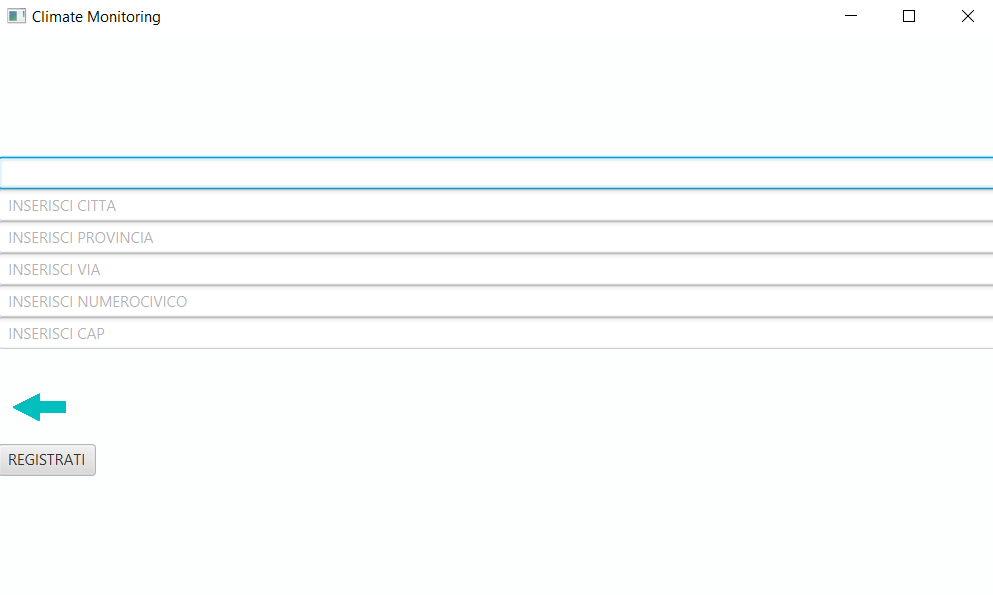
\includegraphics[height=0.3\textheight]{img/utente/NuovoCentroMonitoraggio}
	\caption{Nuovo centro di monitoraggio}
	\label{fig:nuovocentromonitoraggio}
\end{figure}
	
Per completare la registrazione del centro di monitoraggio è possibile selezionare una lista di aree d'interesse associate.

\begin{figure}[h]
	\centering
	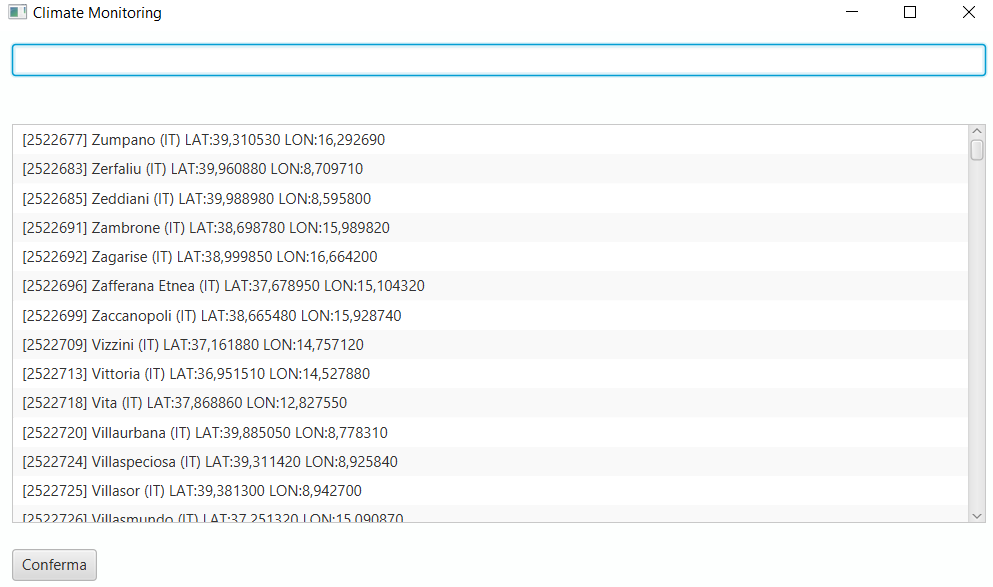
\includegraphics[height=0.3\textheight]{img/utente/SelezioneListaAreeCentroMonitoraggio}
	\caption{Lista Aree}
	\label{fig:selezionelistaareecentromonitoraggio}
\end{figure}

\pagebreak
\subsection{Login}
Nella seguente schermata sono presenti i campi per l'inserimento dei dati per l'accesso dell'operatore.
\begin{figure}[h]
	\centering
	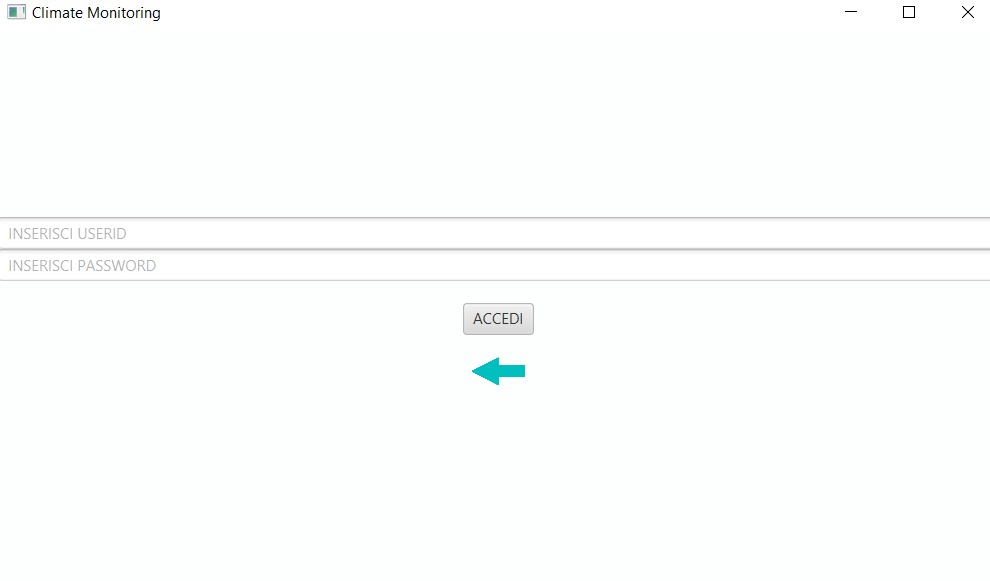
\includegraphics[height=0.3\textheight]{img/utente/Login}
	\caption{Login}
	\label{fig:login}
\end{figure}


In particolare troviamo:
\begin{itemize}
	\item \textbf{UserID} 
	\item \textbf{Password}
\end{itemize} 

Per la conferma è presente il pulsante \textbf{Accedi}.

\pagebreak
\subsection{Inserisci Parametri}
In codesta schermata è presente una barra di ricerca dove l'operatore può selezionare le aree geografiche associate al suo centro di monitoraggio e inserire i punteggi ai vari parametri climatici ed inserire le note relative a quest'ultimi.
Inoltre è presente il tasto invio per salvare tutte le informazioni inserite precedentemente.

\begin{figure}[h]
	\centering
	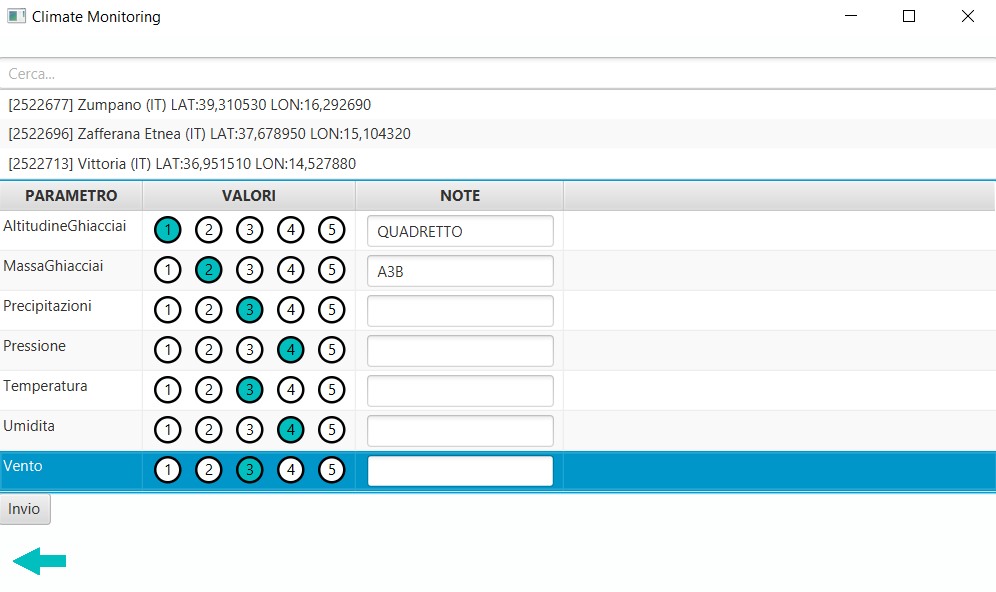
\includegraphics[height=0.3\textheight]{img/utente/InserimentoParametri}
	\caption{Inserimento Parametri}
	\label{fig:inserimentoparametri}
\end{figure}


\subsection{Crea nuovo centro di monitoraggio}
Vedi (Paragrafo \ref{NuovoCentroDiMonitoraggio})
\subsection{Visualizza Aree}
Vedi (Paragrafo \ref{VisualizzaArea} )

\pagebreak
\subsection{Visualizza Profilo} \label{Profilo}
Consente all'operatore registrato di visualizzare i propri dati.

\begin{figure}[h]
	\centering
	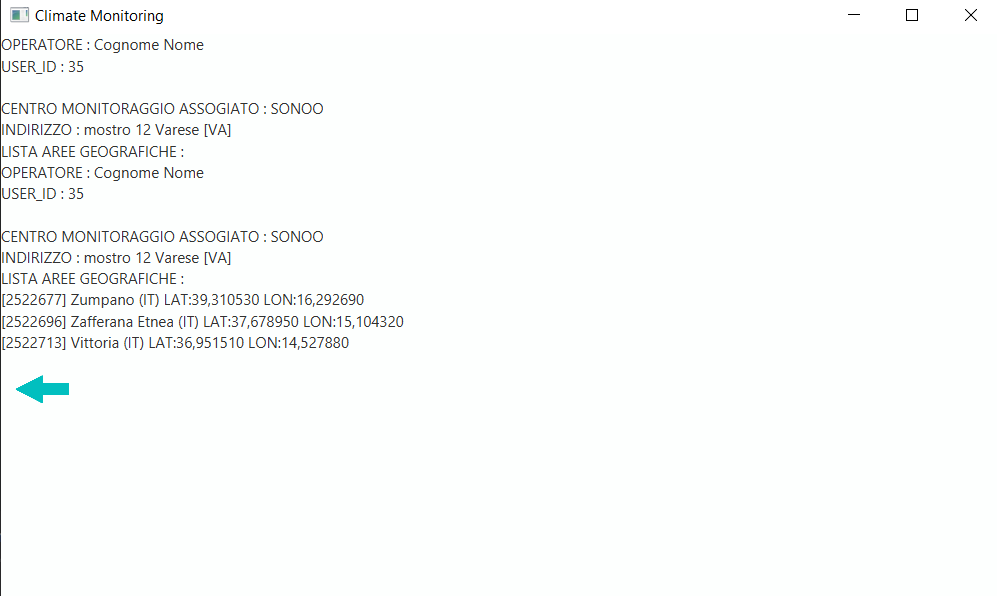
\includegraphics[height=0.3\textheight]{img/utente/VisulizzaProfilo}
	\caption{Visualizza Profilo}
	\label{fig:visulizzaprofilo}
\end{figure}

\subsection{Logout}
Bottone che permette ad un operatore che ha effettuato il login di disconnettersi dal sistema, riportandolo alla schermata home. 

\section{Esci}
Per uscire dall'applicazione è sufficiente chiudere la finestra, cliccando sull'icona a croce ("\textit{Chiudi}" o "\textit{Close}") in alto a destra:

\chapter{Data set di test}
Per testare il funzionamento dell'applicazione sono state inserite nel database al momento della sua creazione alcune istanze di default, tra cui:
\begin{itemize}
	\item Centri di monitoraggio:
	\begin{itemize}
		\item Parco Berrini, Via Roma n.71, 21020, Ternate (VA);
		\item Parco Valle del Lanza, SP20 n.69, 22070, Valmorea (CO);
		\item Golf Club, Via Belmonte n.169, 21100, Induno Olona (VA)
		\item Parco Filo Blu, Via al Collegio n.10,
		28922, Verbania(VCO);
	\end{itemize}
	\item Operatori registrati:
	\begin{itemize}
		\item Beatrice Balzarini, FFHTJN27B59C528G,bbalzarini@studenti.uninsubria.it, pwd: Lampada!23;
		\item Michael Bernasconi, CTAGSM30R50C483Y, mbernasconi@studenti.uninsubria.it, pwd: HikesLover?15;
	\end{itemize}
\end{itemize}



\chapter{Limiti della soluzione sviluppata}
\begin{itemize}
	\item L'istanza del database deve essere l'unica istanza attiva di PostgreSQL, altrimenti il server rischia di connettersi all'istanza sbagliata
	\item A causa della velocità del caricamento delle finestre dell'interfaccia grafica, è necessario premere i vari pulsanti con un singolo click.
	\item E' necessario che l'operatore dopo essersi registrato all'applicazione, si ricordi il proprio userID visualizzabile nella schermata Visualizza Profilo (Paragrafo:\ref{Profilo}), nel caso in cui volesse effettuare login futuri.  
	\item Se si dovesse inserire anche solo un parametro errato nei campi da compilare, l'applicazione mostra un messaggio d'errore generico, che non specifica quale/i dei campi è/sono errato/i.
	\item Si consiglia di non ridimensionare la finestra dell'applicazione in quanto i suoi componenti potrebbero risultare poco ordinati.
\end{itemize}

\nocite{IuriTex}
\bibliographystyle{alpha}
\bibliography{bib/biblio}
